% Illustration of the real-valued non-volume preserving (RNVP) affine coupling layer as introduced in https://arxiv.org/abs/1605.08803.
% Inspired by https://blog.evjang.com/2018/01/nf2.html.

\documentclass[tikz]{standalone}

\usetikzlibrary{calc,positioning}

\begin{document}
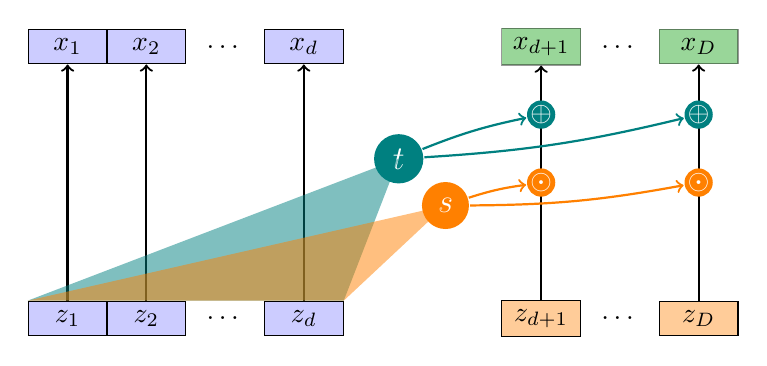
\begin{tikzpicture}[
    thick, text centered,
    box/.style={draw, thin, minimum width=1cm},
    func/.style={circle, text=white},
  ]

  % x nodes
  \node[box, fill=blue!20] (x1) {$x_1$};
  \node[box, fill=blue!20, right of=x1] (x2) {$x_2$};
  \node[right of=x2] (xdots1) {\dots};
  \node[box, fill=blue!20, right of=xdots1] (xd) {$x_d$};
  \node[box, fill=green!60!black, text opacity=1, opacity=0.4, right=2 of xd] (xdp1) {$x_{d+1}$};
  \node[right of=xdp1] (xdots2) {\dots};
  \node[box, fill=green!60!black, text opacity=1, opacity=0.4, right of=xdots2] (xD) {$x_D$};

  % z nodes
  \node[box, fill=blue!20, below=3 of x1] (z1) {$z_1$};
  \node[box, fill=blue!20, right of=z1] (z2) {$z_2$};
  \node[right of=z2] (zdots1) {\dots};
  \node[box, fill=blue!20, right of=zdots1] (zd) {$z_d$};
  \node[box, fill=orange!40, right=2 of zd] (zdp1) {$z_{d+1}$};
  \node[right of=zdp1] (zdots2) {\dots};
  \node[box, fill=orange!40, right of=zdots2] (zD) {$z_D$};

  % z to x lines
  \draw[->] (z1) -- (x1);
  \draw[->] (z2) -- (x2);
  \draw[->] (zd) -- (xd);
  \draw[->] (zdp1) -- (xdp1);
  \draw[->] (zD) -- (xD);

  % scale and translate functions
  \node[func, font=\large, fill=teal, above left=0.1] (t) at ($(zd)!0.5!(xdp1)$) {$t$};
  \fill[teal, opacity=0.5] (z1.north west) -- (t.center) -- (zd.north east) -- (z1.north west);

  \node[func, font=\large, fill=orange, below right=0.1] (s) at ($(zd)!0.5!(xdp1)$) {$s$};
  \fill[orange, opacity=0.5] (z1.north west) -- (s.center) -- (zd.north east) -- (z1.north west);

  % feeding in s and t
  \node[func, inner sep=0, fill=orange] (odot1) at ($(zdp1)!0.5!(xdp1)$) {$\odot$};
  \node[func, inner sep=0, fill=teal] (oplus1) at ($(zdp1)!0.75!(xdp1)$) {$\oplus$};
  \draw[orange, ->] (s) to[bend left=5] (odot1);
  \draw[teal, ->] (t) to[bend left=5] (oplus1);

  \node[func, inner sep=0, fill=orange] (odot2) at ($(zD)!0.5!(xD)$) {$\odot$};
  \node[func, inner sep=0, fill=teal] (oplus2) at ($(zD)!0.75!(xD)$) {$\oplus$};
  \draw[orange, ->] (s) to[bend right=5] (odot2);
  \draw[teal, ->] (t) to[bend right=5] (oplus2);

\end{tikzpicture}
\end{document}